%"###############################################
%
% Classification VAPOR pre 
%
%###############################################

\begin{figure}[H]
\centering
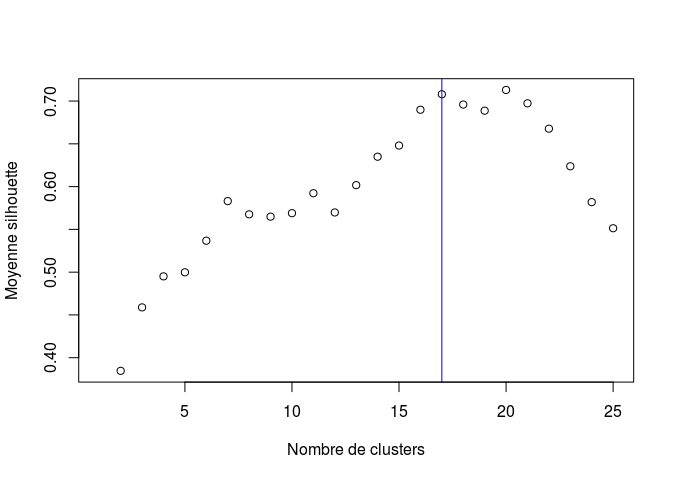
\includegraphics[width=0.90\textwidth]{../Fig/VAPOR/vapor-elbow-pre.png}
\caption{VAPOR Maximise nb cluster / bonne classification}
\end{figure}

\begin{figure}[H]
\centering
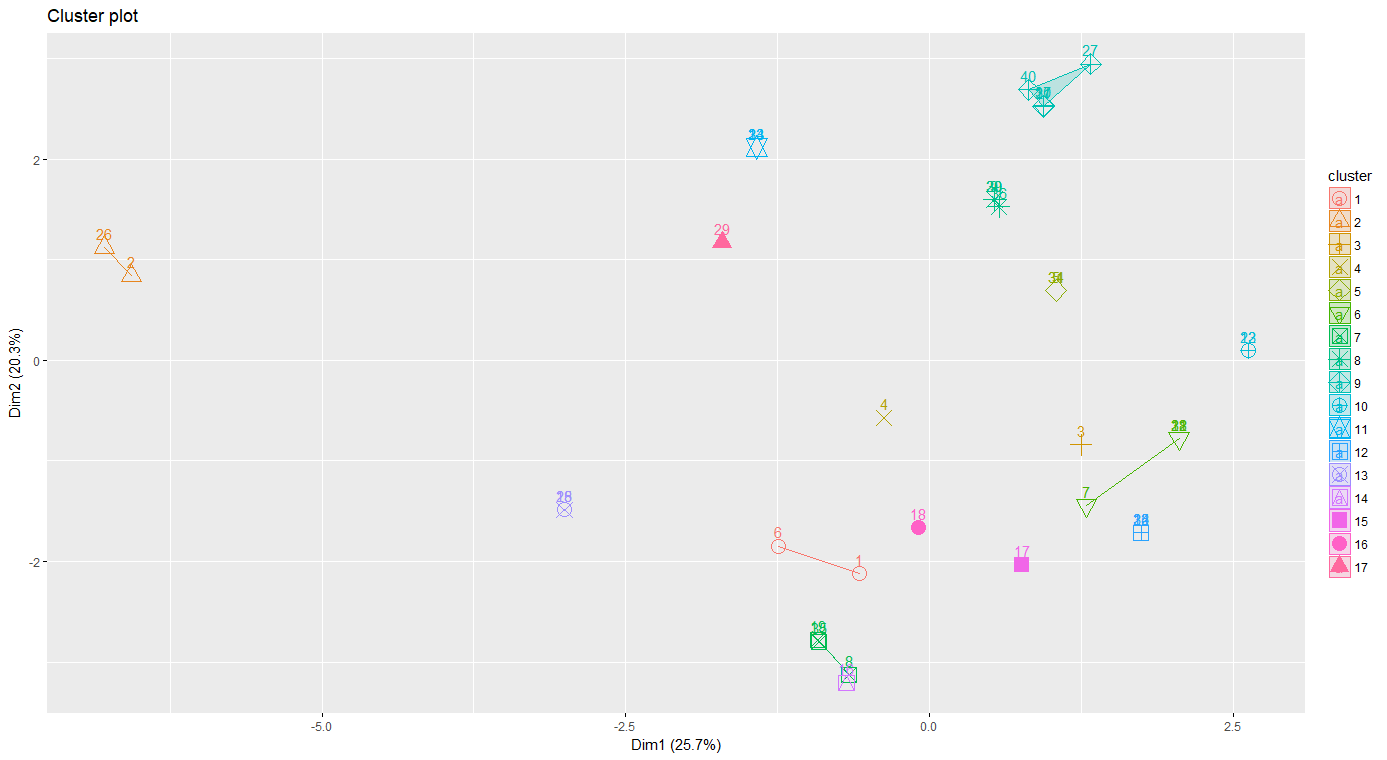
\includegraphics[width=0.90\textwidth]{../Fig/VAPOR/vapor-pam-k17.png}
\caption{VAPOR Nuage de points / clusters PAM k=12 }
\end{figure}

\begin{figure}[H]
\centering
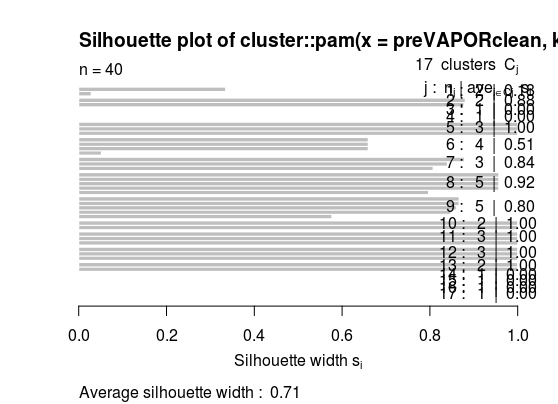
\includegraphics[width=0.90\textwidth]{../Fig/VAPOR/vapor-sil-pre.png}
\caption{VAPOR silhouette / clusters PAM k=17 }
\end{figure}

%\begin{figure}[H]
%\centering
%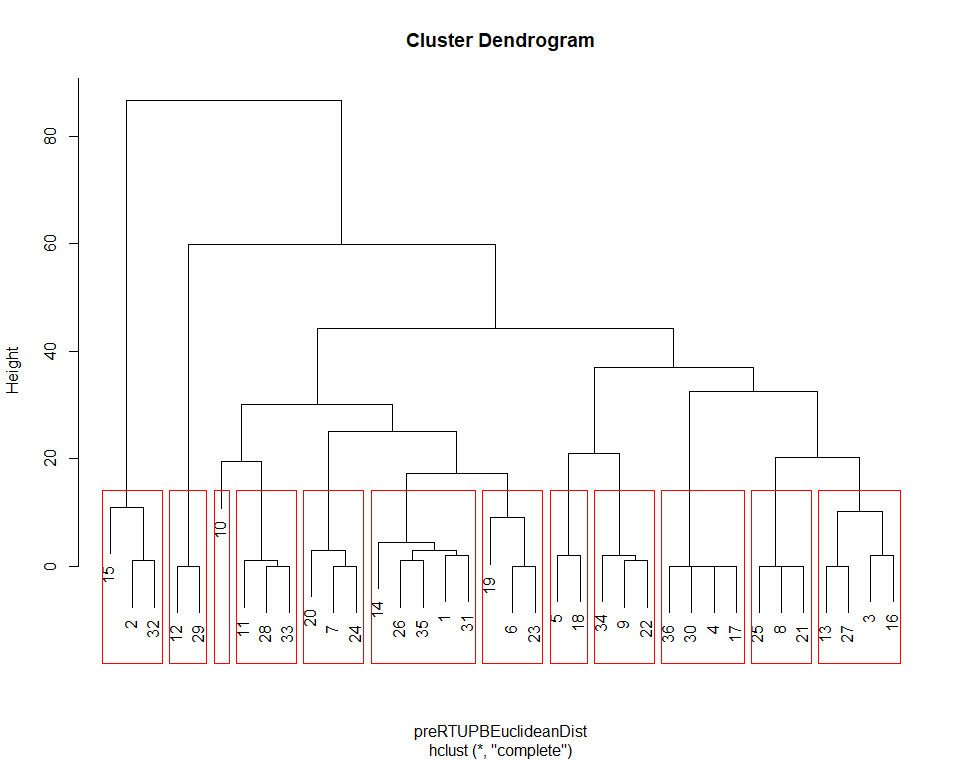
\includegraphics[width=0.90\textwidth]{../Fig/RTUPB/rtupb-cah-k12-pre.png}
%\caption{RTUPB CAH séparation en k=12 }
%\end{figure}


%"###############################################
%
% Interpretation des trois figures VAPOR pre 
%
%#############################################




%\begin{figure}[h]
%    \begin{minipage}[c]{.46\linewidth}
%        \centering
%        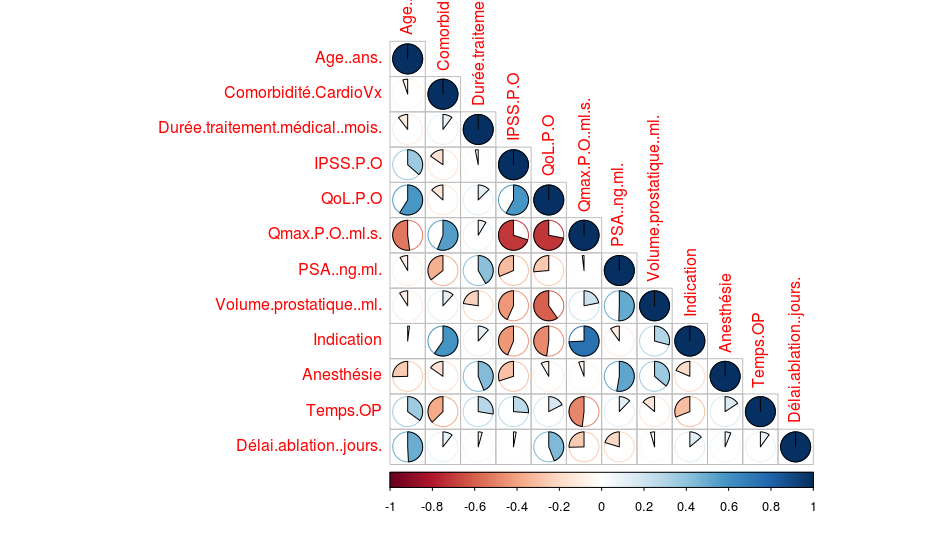
\includegraphics[width=1\textwidth]{../Fig/VPPBS/vppbs-corr-matrice-pie}
%        \caption{Légende}
%    \end{minipage}
%    \hfill%
%    \begin{minipage}[c]{.46\linewidth}
%        \centering
%        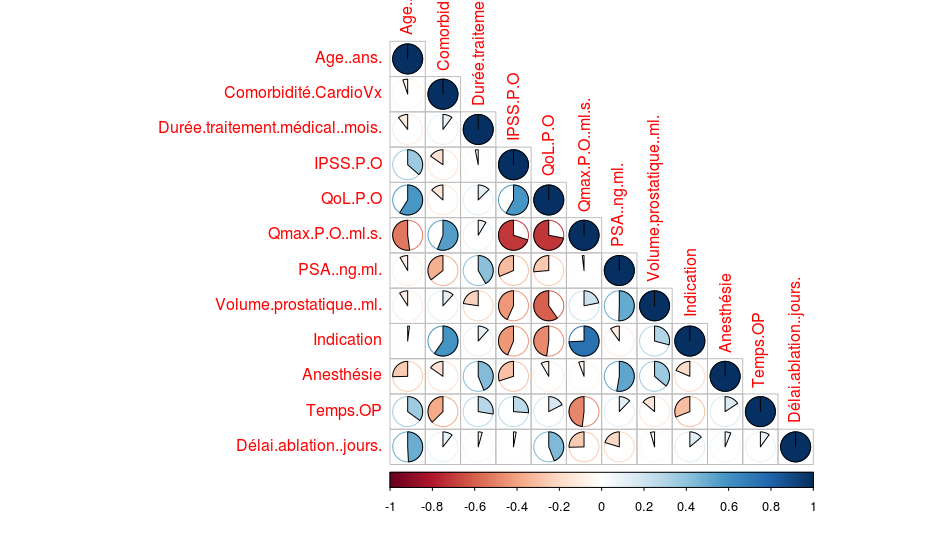
\includegraphics[width=1\textwidth]{../Fig/VPPBS/vppbs-corr-matrice-pie}
%        \caption{Légende}
%    \end{minipage}
%\end{figure}





%
%##########################
%# CONCLUSION
%##########################
